\documentclass[pdf,11pt]{beamer}

\usepackage[utf8]{inputenc}
\usepackage{graphicx}       % Images
\graphicspath{{Images/}}
\usepackage{xcolor}         % Change Colors
\usepackage{caption}
\captionsetup[figure]{font=small}
\usepackage{multimedia}     % Movies!
\usepackage{tikz}           % Vectored pictures
%\usepackage{media9}
\hypersetup{pdfpagemode=FullScreen} % Presentation Mode

% Remove navigation symbols
\beamertemplatenavigationsymbolsempty
% Add page number
\addtobeamertemplate{navigation symbols}{}{%
    \usebeamerfont{footline}%
    \usebeamercolor[fg]{footline}%
    \hspace{1em}%
    \insertframenumber/\inserttotalframenumber
}

% Title
\title{Research and Applications of Scientific Visualization
    %\small A Granular Analysis of Neural Machine Translation Architectures
}
\author{Steven Walton\\ \small University of Oregon}
\date{10 Mar 2020}

\usebackgroundtemplate
{
    
\includegraphics[width=\paperwidth,height=\paperheight]{UO_Simple.png}
}
\definecolor{UOYellow}{HTML}{FDCB00}
\definecolor{UOGreen}{HTML}{424443}
%\newcommand{\mytitle}[1]{\setcolor{bg=UOYellow,fg=green}\frametitle{{#1}}}

% Formatting
%   \setbeamercolor{title}{fg=white}
%   \setbeamercolor{normal text}{fg=white}
%   \setbeamercolor{structure}{fg=white}        % Adjusts figures and frame titles
%   \setbeamertemplate{frametitle}[default][center]
%   \setbeamerfont{frametitle}{size=\Huge}
%   %\setbeamerfont{normal text}{size=\LARGE}
%   %\setbeamerfont{structure}{size=\LARGE}
%   \setbeamercolor{footline}{fg=UOGreen}
%   %\setbeamerfont{footline}{series=\bfseries}


\begin{document}
\frame{\titlepage}

\begin{frame}
\frametitle{Overview}
    \begin{itemize}
        \item \emph{\color{UOYellow}Background}
        \item Methodology 
        \item Results
        \item Future Work
    \end{itemize}
\end{frame}

\begin{frame}
\frametitle{Background}
    \begin{itemize}
        \item Growth in compute speed in supercomputers is out pacing growth in
            IO speed and storage by 10 to 1.
        \item Supercomputers are generating so much data so fast that we cannot
            save it fast enough and do not have enough storage to save high
            resolution time series data.
        \item Simulation science is exploratory by nature. We don't always know
            what we want a priori (beforehand)
        \item Interesting events can happen between save states.
    \end{itemize}
\end{frame}

\begin{frame}
\frametitle{What We Need}
    \begin{itemize}
        \item Need to be able to explore the simulation in situ.
        \item Need to be able to extract information across large time steps
            while saving data infrequently. 
    \end{itemize}
\end{frame}

\begin{frame}
    \frametitle{What Has Been Done}
    \begin{itemize}
        \item Conventionally scientists LERP between timesteps.
        \item Current research is into different machine learning models to
            infer data between timesteps. 
    \end{itemize}
\end{frame}

\begin{frame}
\frametitle{TSR-TVD: Temporal Super-Resolution for Time-Varying Data Analysis and
    Visualization}
    \begin{itemize}
        \item HPC has issues with storing time-steps.
        \item Some researchers LERP between time-steps to find intermediate
        data.
        \item TSR-TVD is a machine learning implementation to synthesize
        timesteps.
        \item Researchers are modifying existing ML techniques to solve problems
        in HPC.
        \item https://ieeexplore.ieee.org/document/8802285
    \end{itemize}
\end{frame}

\begin{frame}
\frametitle{TSR-TVD: Temporal Super-Resolution for Time-Varying Data Analysis and
    Visualization}
    \center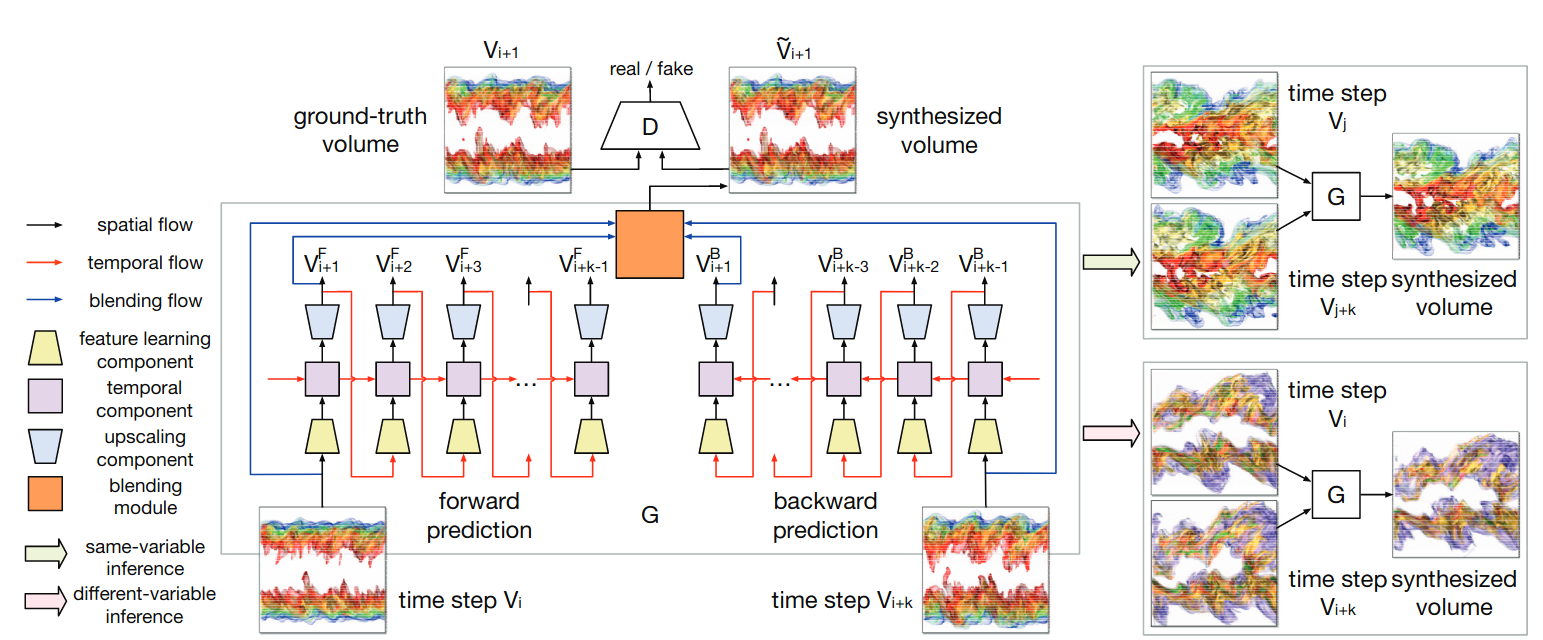
\includegraphics[width=0.9\paperwidth]{TSR.png}
\end{frame}

\begin{frame}
\frametitle{TSR-TVD: Temporal Super-Resolution for Time-Varying Data Analysis and
    Visualization}
    \begin{itemize}
        \item Uses RNN to create forward and backward predictions
        \item Conv3D GAN adversarially trains network.
        \item TSR-TVD uses structure similar to TecoGAN
    \end{itemize}
\end{frame}

\begin{frame}
\frametitle{TSR-TVD: Temporal Super-Resolution for Time-Varying Data Analysis and
    Visualization}
    \center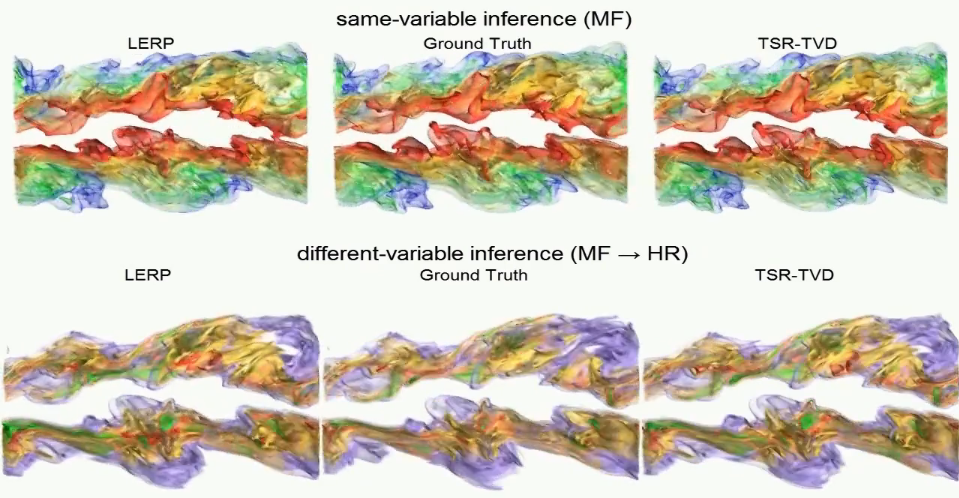
\includegraphics[width=0.8\paperwidth]{TSR_Link.png}
    \\
    \href{https://vimeo.com/359998660}{Short Video}\\ 
    https://vimeo.com/359998660
\end{frame}

\begin{frame}
\frametitle{TSR-TVD: Temporal Super-Resolution for Time-Varying Data Analysis and
    Visualization}
    \center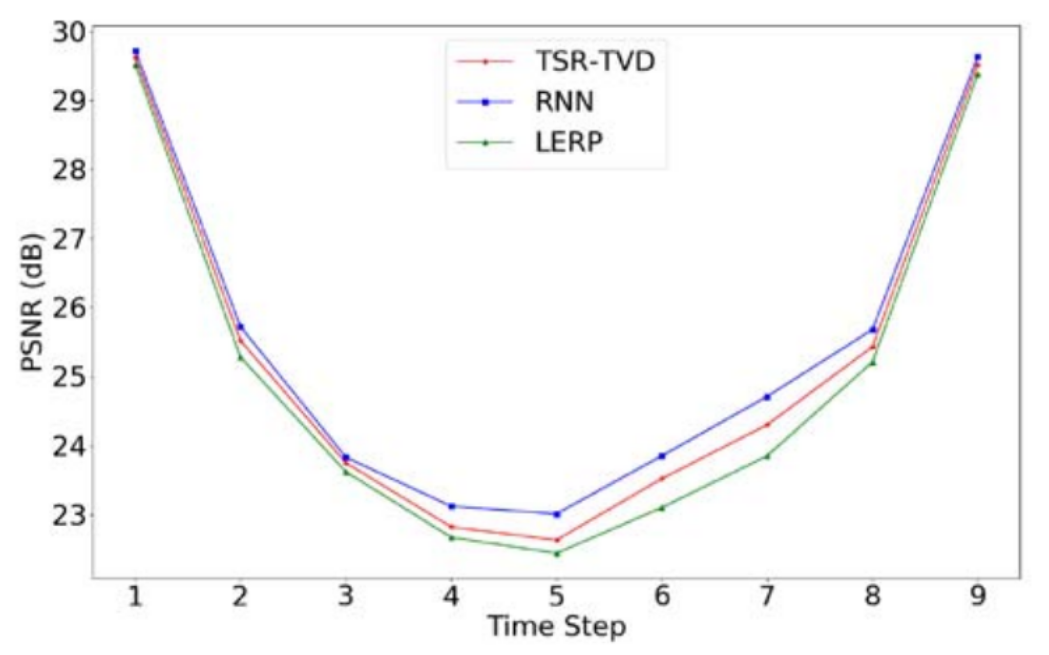
\includegraphics[width=0.8\paperwidth]{PSNR.png}
\end{frame}


\begin{frame}
\frametitle{Overview}
    \begin{itemize}
        \item \emph{\color{UOYellow}Background}
        \item Methodology 
        \item Results
        \item Future Work
    \end{itemize}
\end{frame}

\begin{frame}
\frametitle{Background}
    \begin{itemize}
        \item Growth in compute speed in supercomputers is out pacing growth in
            IO speed and storage by 10 to 1.
        \item Supercomputers are generating so much data so fast that we cannot
            save it fast enough and do not have enough storage to save high
            resolution time series data.
        \item Simulation science is exploratory by nature. We don't always know
            what we want a priori (beforehand)
        \item Interesting events can happen between save states.
    \end{itemize}
\end{frame}

\begin{frame}
\frametitle{What We Need}
    \begin{itemize}
        \item Need to be able to explore the simulation in situ.
        \item Need to be able to extract information across large time steps
            while saving data infrequently. 
    \end{itemize}
\end{frame}

\begin{frame}
    \frametitle{What Has Been Done}
    \begin{itemize}
        \item Conventionally scientists LERP between timesteps.
        \item Current research is into different machine learning models to
            infer data between timesteps. 
    \end{itemize}
\end{frame}

\begin{frame}
\frametitle{Diamonds That Deliver}
\begin{columns}
    \begin{column}{0.5\paperwidth}
    \begin{itemize}
        \item HPC simulations are used to solve complex problems such as drug
        delivery.
        \item Theory suggests that nanodiamonds are good delivery candidates.
        \item ORNL researchers were able to simulate tRNA transfer without
        having to test on humans.
        \item This work was done on Titan.
        \item
        \href{https://pubs.acs.org/doi/full/10.1021/acs.jpcb.6b07511}{https://pubs.acs.org/doi/full/10.1021/acs.jpcb.6b07511}
    \end{itemize}
    \end{column}
    \begin{column}{0.5\paperwidth}
        \center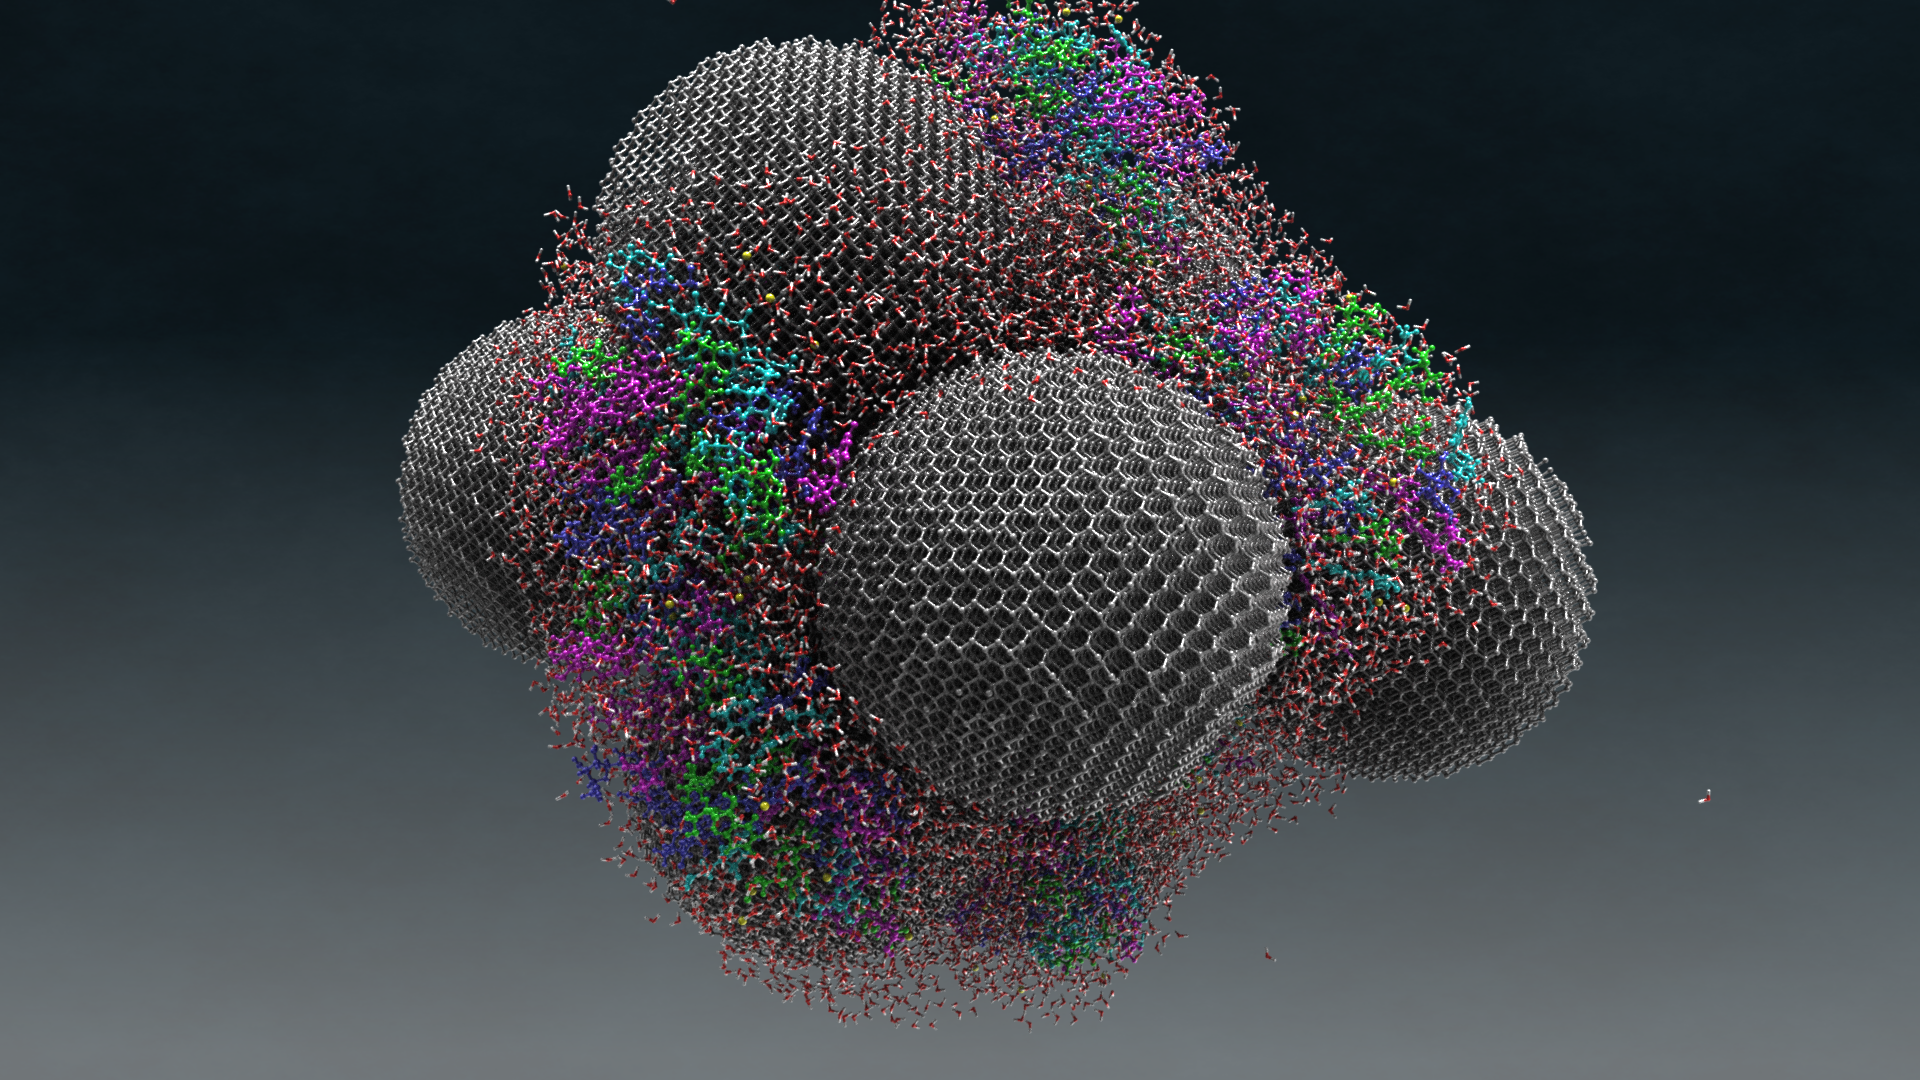
\includegraphics[width=0.8\textwidth]{NanoDiamond.png}
    \end{column}
\end{columns}
\end{frame}

\begin{frame}
\frametitle{Diamonds That Deliver}
\center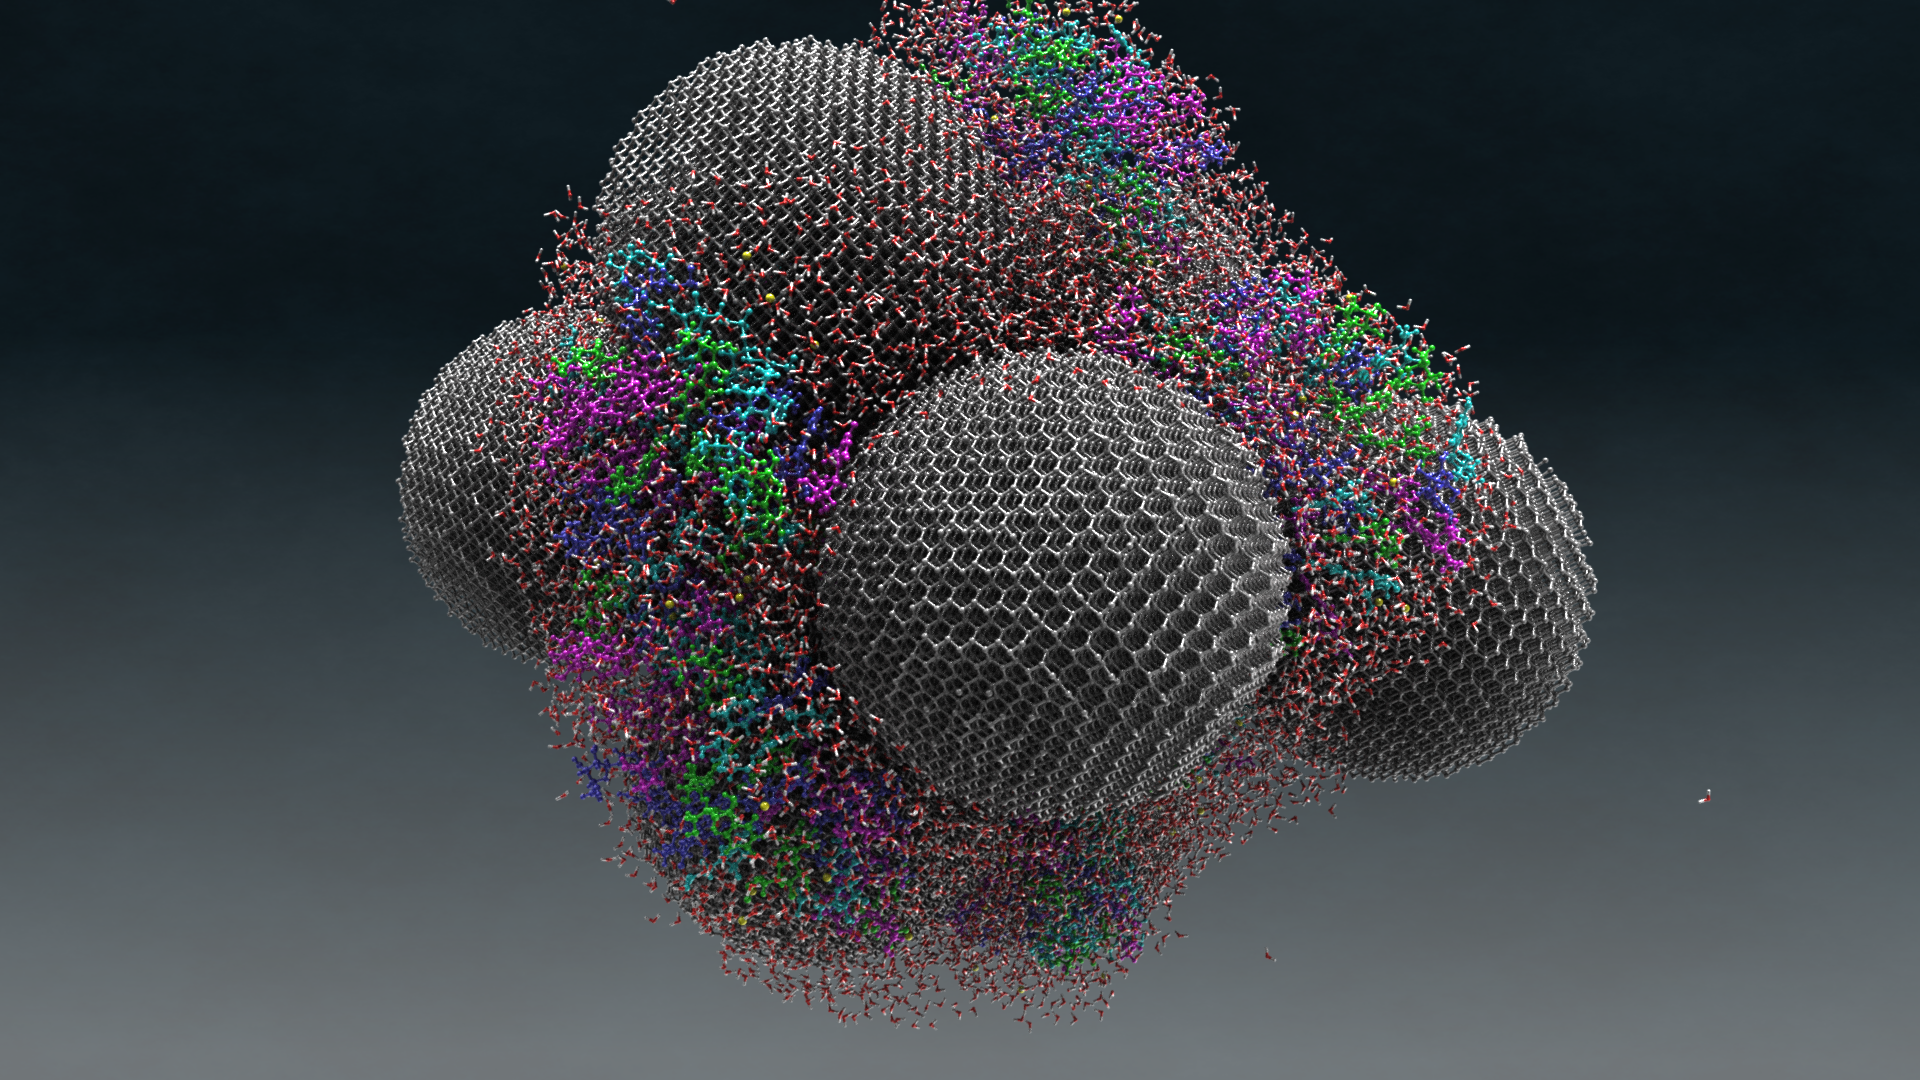
\includegraphics[width=\textwidth]{NanoDiamond.png}
\end{frame}

\begin{frame}
\frametitle{Diamonds That Deliver}
\center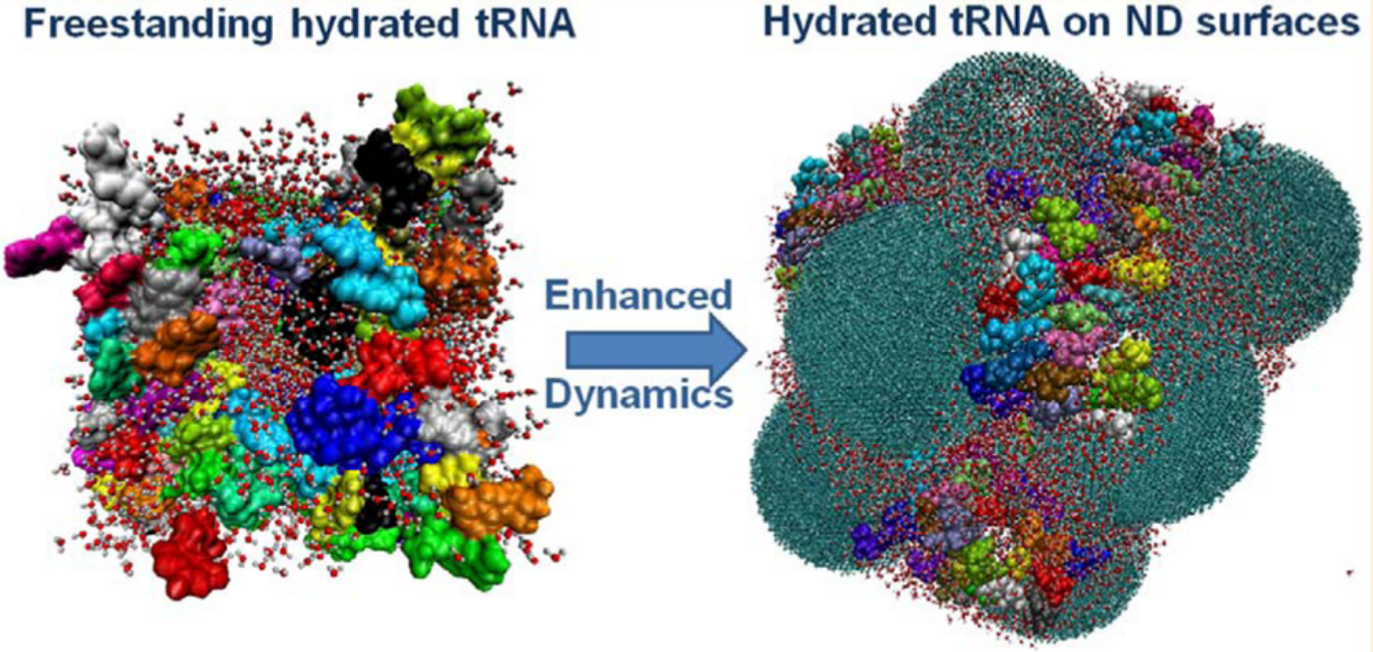
\includegraphics[width=\textwidth]{hydrated_tRNA.png}
\end{frame}

\begin{frame}
\frametitle{Diamonds That Deliver}
\center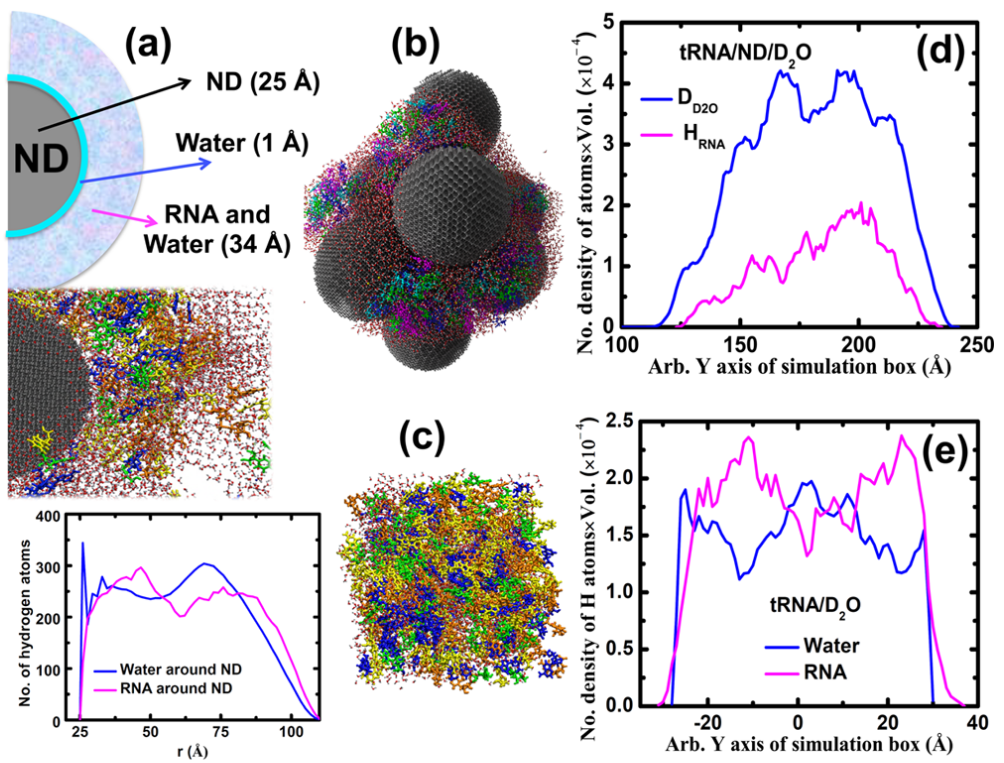
\includegraphics[width=\textwidth]{tRNA_analysis.png}
\end{frame}

\begin{frame}
\frametitle{Diamonds That Deliver}
    \begin{itemize}
        \item
        \href{https://www.youtube.com/watch?v=59428CbAXWE}{https://www.youtube.com/watch?v=59428CbAXWE}
        \item
        \href{https://www.youtube.com/watch?v=w4wQGXfEoMg}{https://www.youtube.com/watch?v=w4wQGXfEoMg}
    \end{itemize}
\end{frame}

\begin{frame}
\frametitle{Diamonds That Deliver}
    \begin{itemize}
        \item The visualizations are what lead to better understanding.
        \item Let's scientists "quickly" determine drug candidates and delivery
        mechanisms.
        \item These simulations helped inform scientists of the motions of tRNA
        and this helps them treat conditions such as cancer and genetic
        disorders.
        \item ORNL is currently using Summit to screen drugs for the Corona
        Virus.
    \end{itemize}
\end{frame}


\end{document}
